% Especificaciones del tamaño de letra, tamaño de hoja, márgenes, librerias, etc.
\documentclass[12pt, letterpaper]{article}
\usepackage[english]{babel}
\usepackage{fancyhdr}
\usepackage[utf8]{inputenc}
\usepackage[T1]{fontenc}
\usepackage{amsmath}
\usepackage{graphicx}
\usepackage{subcaption}
\usepackage[hidelinks]{hyperref}
\usepackage{url}
\usepackage{amssymb}
\usepackage{float}
\usepackage[margin=1in]{geometry}
\renewcommand{\baselinestretch}{1.5}

% Enlace Bibliografía
\usepackage{csquotes}
\usepackage[notes,backend=biber]{biblatex-chicago}
\addbibresource{referencias.bib}

% Titulo, autores, fecha.
\title{Technical Report \#2}
\author{Carlos A. Vásquez Castañeda \and 1155057 \and Group 392}
\date{December 4, 2019}
\pagestyle{fancy}
\fancyhf{}
\rhead{Aircraft Elements Design}
\lhead{Technical Report \#2}
\rfoot{\thepage}


% Inicio del documento
\begin{document}
\maketitle
\section*{Introduction}

As with the assembly of the individual modules and components of the engine, the casing is of huge importances as it will carry the whole engine and the proper assembly will secure it. If there is a flaw in the system, such as an unexpected obstruction, the fan blade can brake, spin off, and harm other engine components. Fan casings, therefore, need to be strong enough to contain errant blades and damage-tolerant to withstand the punishment of a loose blade-turned-projectile. \autocite{spinoffnasa}

\section*{Assembly}

The first thing we did was to import all the casings that were needed. A particularity of the casings was that they all were done with a shaft technique, so trying to make a coincidence via concentricity was not possible. Therefore the solution is to align the planes. This way, the orientation and rotation of the casings is locked. This is similar to the way the combustor was constrained and it only had one degree of freedom left. In figures 1 and 2 the planes that are constrained are shown in dotted blue lines. In this manner, the planes of the casings were constrained with the fixed planes of the shaft.

\begin{figure}[H]
	\centering
	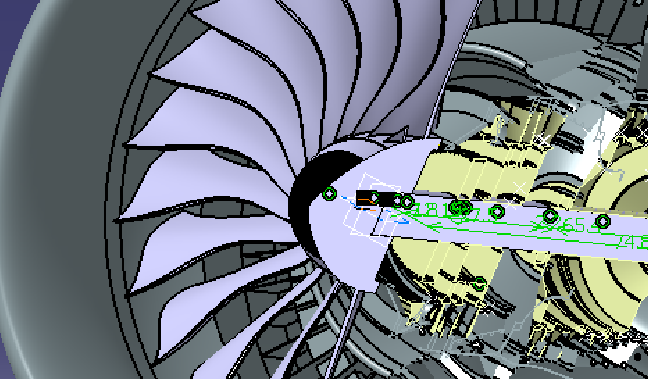
\includegraphics[width=0.7\textwidth]{1.png}
	\caption{Coincidence of the plane xy.}
\end{figure}

\begin{figure}[H]
	\centering
	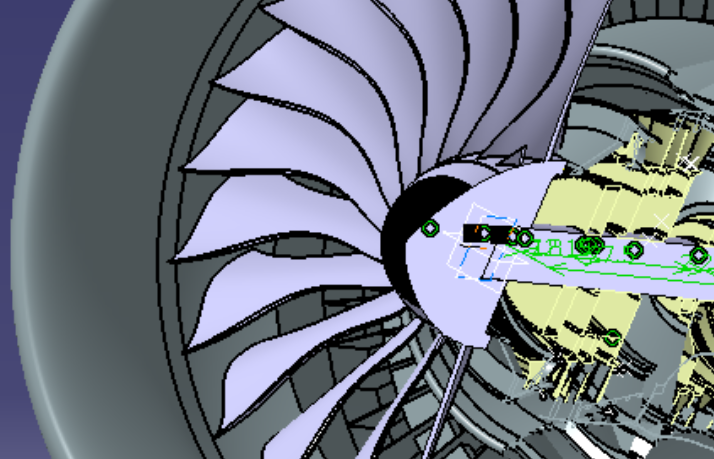
\includegraphics[width=0.7\textwidth]{2.png}
	\caption{Coincidence of the plane yz.}
\end{figure}

This procedure was followed with every other casing in order to constrain the components of the casing as a whole. After all the parts of the casing were constrained in the same axis, the next part was to connect them together. The way this was done was by the coincidence of the faces of the different parts of the casing. These individual components were designed so every face of every other component had a cross section that faced the cross section of the other component. This makes the assembly process easier. In the figures below is shown the different coincidence constrains made with each individual component.

\begin{figure}[H]
	\centering
	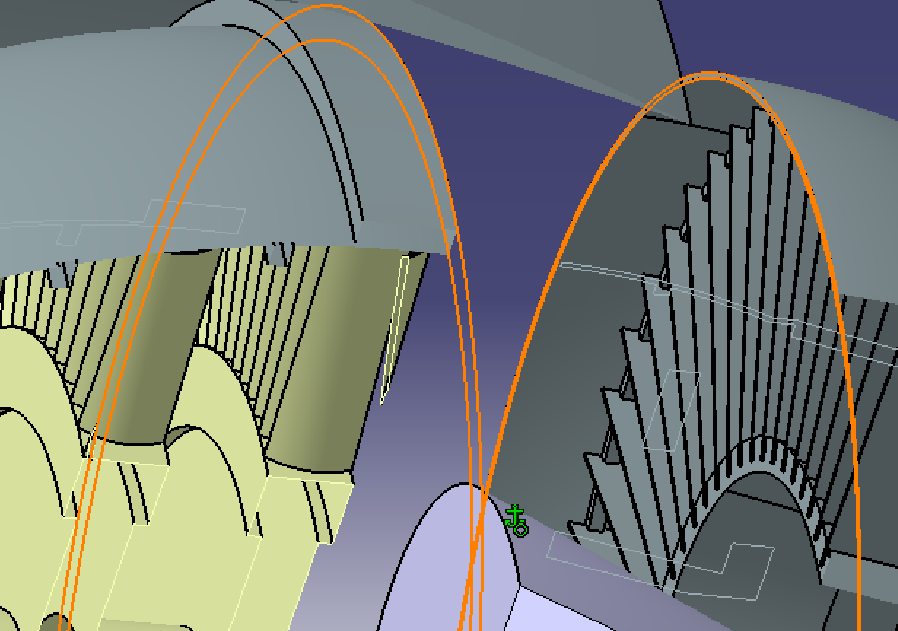
\includegraphics[width=0.7\textwidth]{3.png}
	\caption{Coincidence of cross sections. Turbine case and exhaust case shown in the photo. Cross sections shown in orange.}
\end{figure}

\begin{figure}[H]
	\centering
	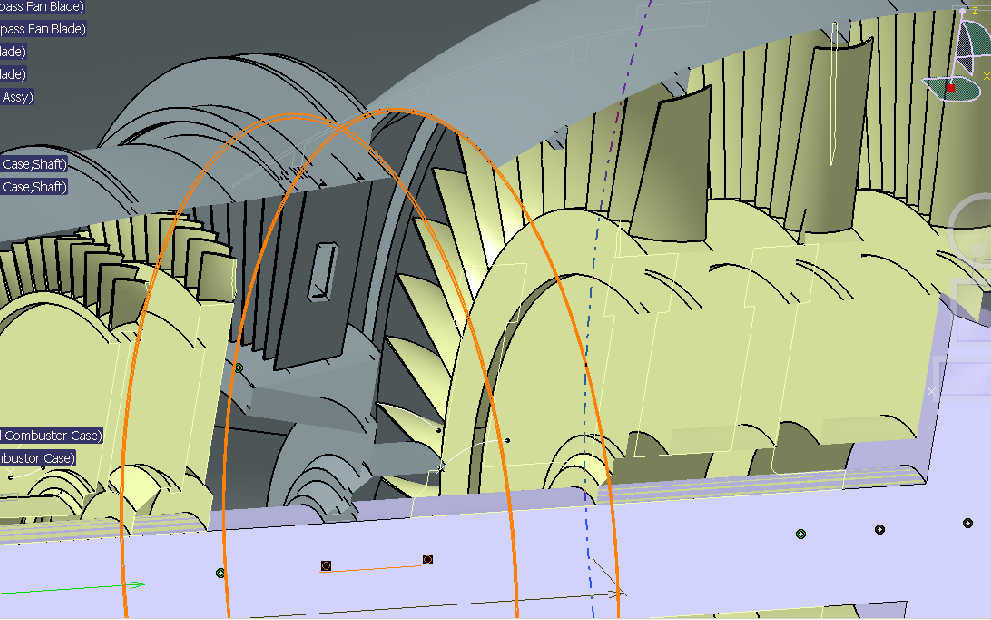
\includegraphics[width=0.7\textwidth]{4.png}
	\caption{Coincidence of cross sections between the inlet guide vanes turbine (IGV Turbine) and the turbine case, shown in orange.}
\end{figure}

\begin{figure}[H]
	\centering
	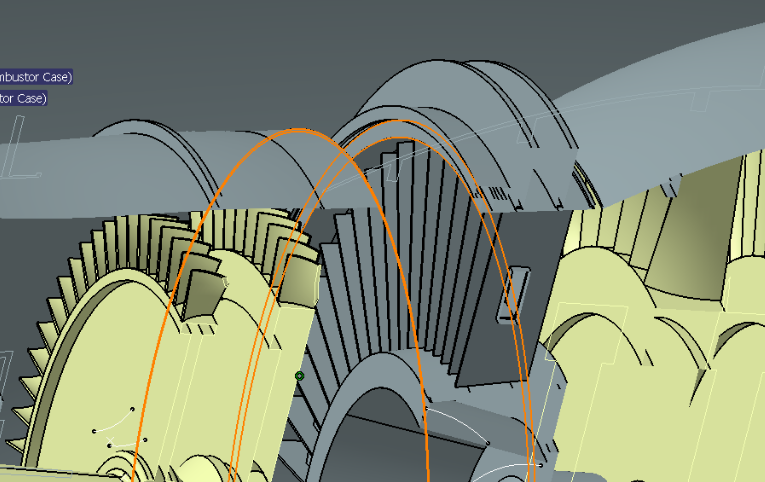
\includegraphics[width=0.7\textwidth]{5.png}
	\caption{Coincidence of cross sections between the IGV turbine and the compressor and combustor case, shown in orange.}
\end{figure}

\begin{figure}[H]
	\centering
	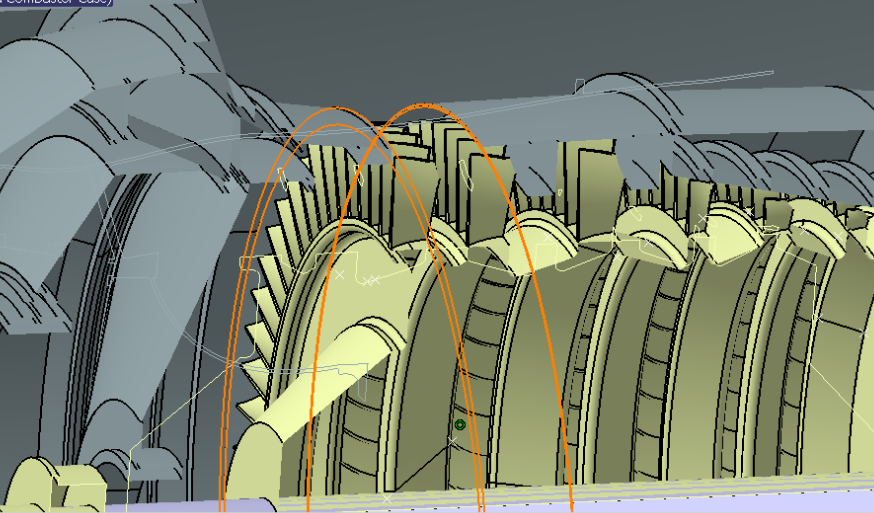
\includegraphics[width=0.7\textwidth]{6.png}
	\caption{Coincidence of cross sections between the nacelle and the compressor and combustor case, shown in orange.}
\end{figure}


Although most of the assembly is complete, there are some things left to do. The casing for the planetary assembly is not related to any other casing the same way the others are, so it is not possible to make a relationship with them. The way this can be solved is by making an offset constrain relative to a fixed point (like how the offsets for the different pieces inside the engine were made). 

\begin{figure}[H]
	\centering
	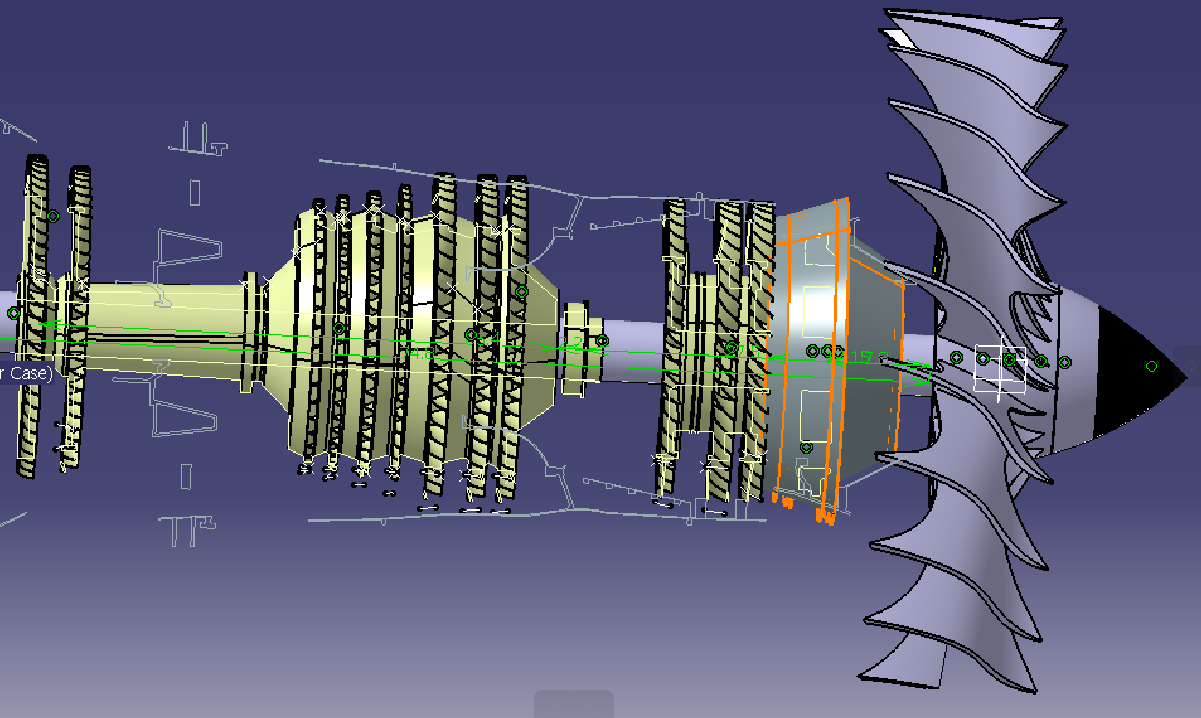
\includegraphics[width=0.7\textwidth]{7.png}
	\caption{Planetary gear assembly casing view from the side.}
\end{figure}

\begin{figure}[H]
	\centering
	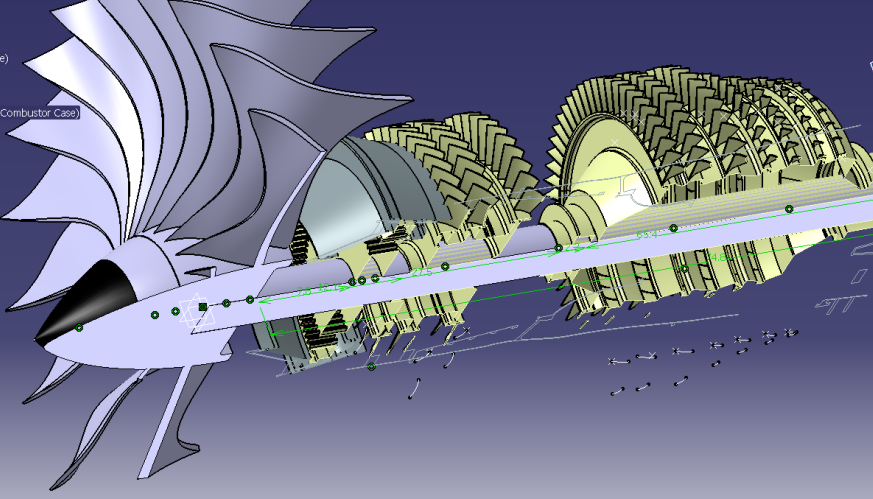
\includegraphics[width=0.7\textwidth]{8.png}
	\caption{Cross section of the planetary gear assembly case.}
\end{figure}

As with the planetary gear assembly case, the combustor falls into the same problem, and the way of solving is similar, as it only needs one more restriction to fall in place properly.

\section*{Conclusion}

Since the only things left to constrain are the offsets of the planetary gear, the combustor and the nacelle (relative to a fixed point), the assembly of the engine as a whole is more or less finished, with a few things that should be checked. For instance, after creating every constrain we must check if there is not a constrain which is inconsistent or if the assembly is overconstrained. Also, as the different parts will rotate and move, we should make sure that there is not a clash between the components of the engine. After this, we might say that the assembly is secured and finished.

\begin{figure}[H]
	\centering
	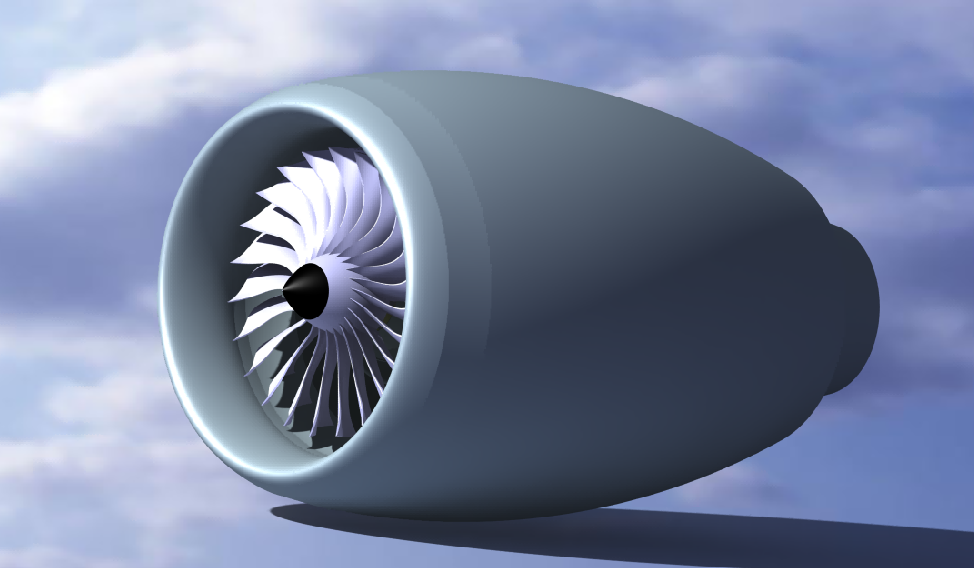
\includegraphics[width=0.7\textwidth]{rend.png}
	\caption{Render of the engine and the casings.}
\end{figure}

\begin{figure}[H]
	\centering
	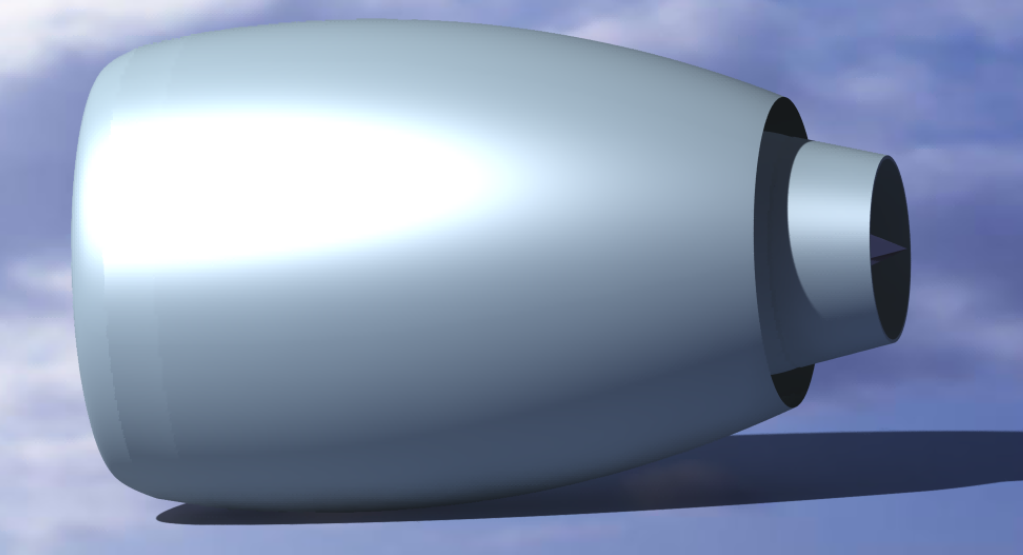
\includegraphics[width=0.7\textwidth]{rends.png}
	\caption{Sideview of the casings.}
\end{figure}

\begin{figure}[H]
	\centering
	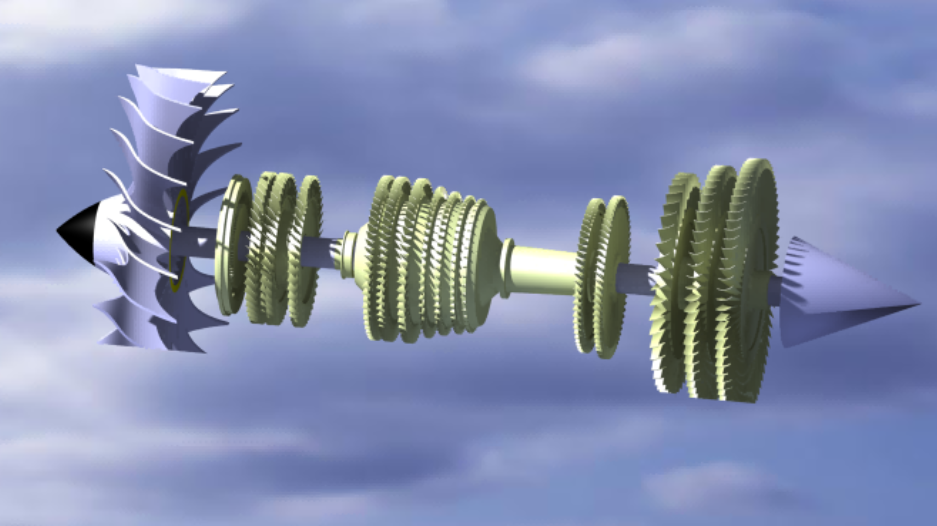
\includegraphics[width=0.7\textwidth]{rend4.png}
	\caption{The insides of the engine.}
\end{figure}

\begin{figure}[H]
	\centering
	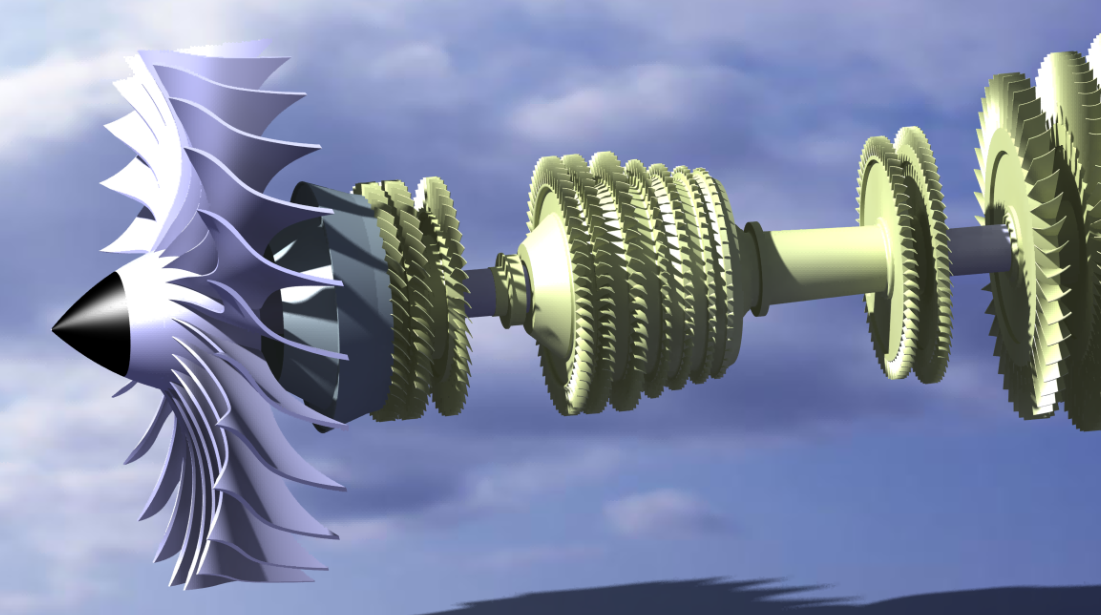
\includegraphics[width=0.7\textwidth]{rend5.png}
	\caption{Render of the inside of the engine with the planetary gear assembly case.}
\end{figure}
%%%%%  Bib
\renewcommand\refname{References}
\printbibliography

\end{document}
